%NEEDSequg
%tabspektrum, tabaall, tabay, tabug, tabalinreg, picaALL, picavio2lin, picavio1lin, picagrunlin, picagelblin, picablaugrunlin, picblinreg1

\subsection{Bestimmung von $U_g$} %Abhängigkeit des Photostromes von Bremsspannung}
\begin{table}[h]
	\begin{center}
		\begin{tabular}{ccc}
			$\lambda$/nm&Farbe&$\nu \cdot 10^{(14)}$/$\frac{1}{\text{s}}$ \\ \hline
			405&Violett&7,40\\
			435&Violett&6,89\\
			492&Grün&6,09\\
			546&Blaugrün&5,49\\
			578&Gelb&5,19
		\end{tabular}
		\caption{Untersuchte Linien des Hg-Spektrums[1]}
		\label{tabspektrum}
	\end{center}
\end{table} \begin{table}[h]
	\begin{center}
		\begin{tabular}{c|cccc}
			$U$/V&405nm: I/nA&435nm: I/nA&492nm: I/nA&546nm: I/nA \\ \hline
			-1,0&	0,027& 0,000&0,000&-0,018\\
			-0,8&	0,097& 0,094&0,000&-0,016\\
			-0,6&	0,225& 0,280&0,003&-0,011\\
			-0,4&	0,400& 0,720&0,012& 0,011\\
			-0,2&	0,630& 1,100&0,030& 0,140\\
			 0,0&	0,840& 1,350&0,054& 0,460\\
			 0,2&	1,050& 2,050&0,080& 0,830\\
			 0,4&	1,350& 2,550&0,105& 1,200\\
			 0,6&	1,650& 3,100&0,135& 1,500\\
			 0,8&	1,900& 3,600&0,155& 1,800\\
			 1,0&	2,200& 4,000&0,175& 2,050\\
			 5,0&	7,200&12,500&0,530& 5,600\\
			 9,0&  10,000&17,500&0,720& 7,000\\
			13,0&  12,000&20,500&0,820& 7,800\\
			17,0&  13,500&22,500&0,870& 8,200\\
			19,0&  14,000&23,000&0,930& 8,700
		\end{tabular}
		\caption{Photostrom verschiedener Wellenlängen in Abhängigkeit der Spannung}
		\label{tabaall}
	\end{center}
\end{table} \begin{table}[h]
	\begin{center}
		\begin{tabular}{cc}
			$U_g$/V&I/nA \\ \hline
			-19,0&-0,010\\
			-17,0&-0,012\\
			-13,0&-0,011\\
			 -9,0&-0,009\\
			 -5,0&-0,009\\
			 -1,0&-0,008\\
			 -0,8&-0,006\\
			 -0,6&-0,004\\
			 -0,4&0,000\\
			 -0,2&0,018\\
			  0,0&0,120\\
			  0,2&0,290\\
			  0,4&0,460\\
			  0,6&0,610\\
			  0,8&0,720\\
			  1,0&0,880\\
			  5,0&1,800\\
			  9,0&2,200\\
			 13,0&2,350\\
			 17,0&3,800\\
			 19,0&4,000
		\end{tabular}
		\caption{Photostrom in Abhängigkeit der Spannung ($\lambda=578$ nm)}
		\label{tabay}
	\end{center}
\end{table} 	\begin{figure}[h]
		\begin{center}
		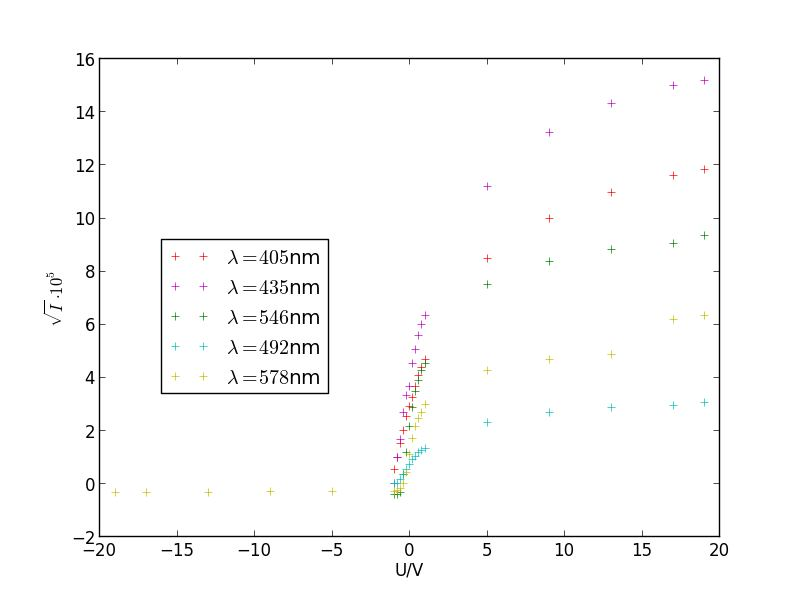
\includegraphics[scale=0.7]{picaALL.jpg}
		\caption{Photostrom in Abhängigkeit der angelegten Spannung}
		\label{picaALL}
		\end{center}	
	\end{figure}
	\begin{figure}[h]
		\begin{center}
		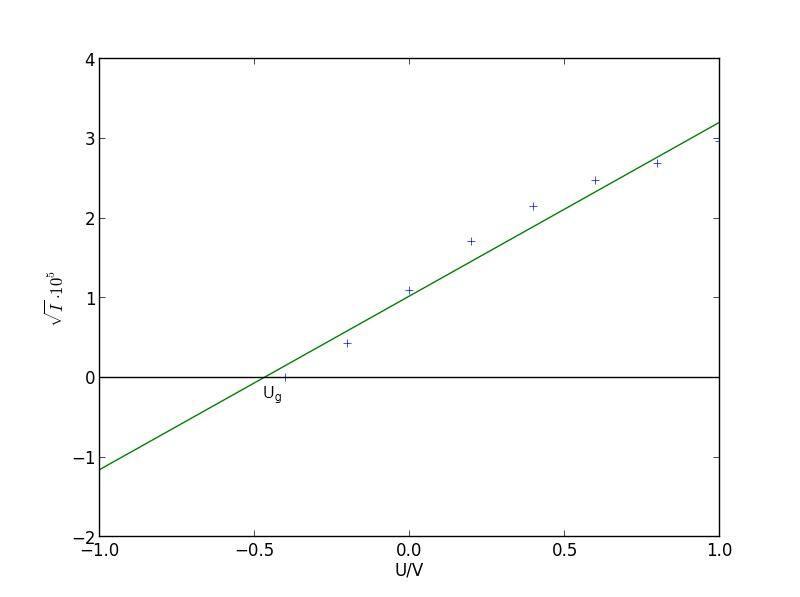
\includegraphics[scale=0.7]{picagelblin.jpg}
		\caption{Lineare Regression des Photostroms ($\lambda=578$ nm)}
		\label{picagelblin}
		\end{center}	
	\end{figure} 	\begin{figure}[h]
		\begin{center}
		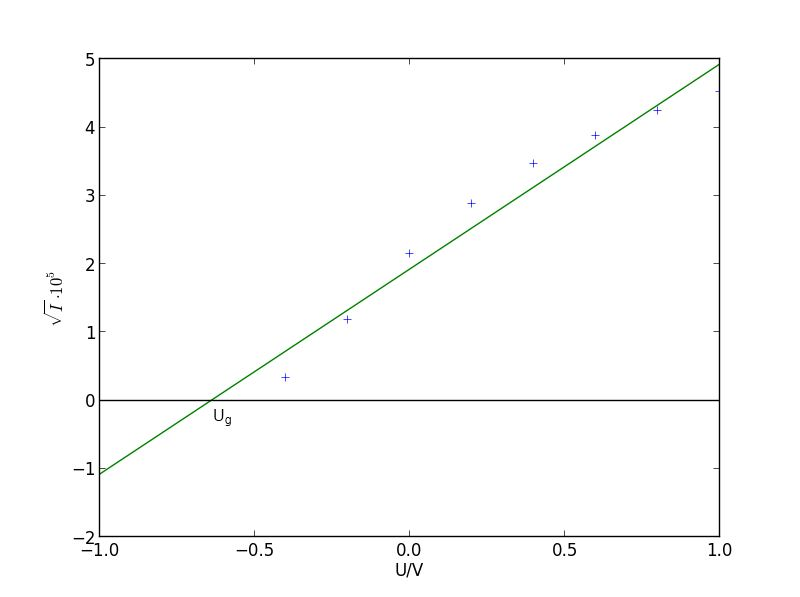
\includegraphics[scale=0.7]{picagrunlin.jpg}
		\caption{Lineare Regression des Photostroms ($\lambda=546$ nm)}
		\label{picagrunlin}
		\end{center}	
	\end{figure} 	\begin{figure}[h]
		\begin{center}
		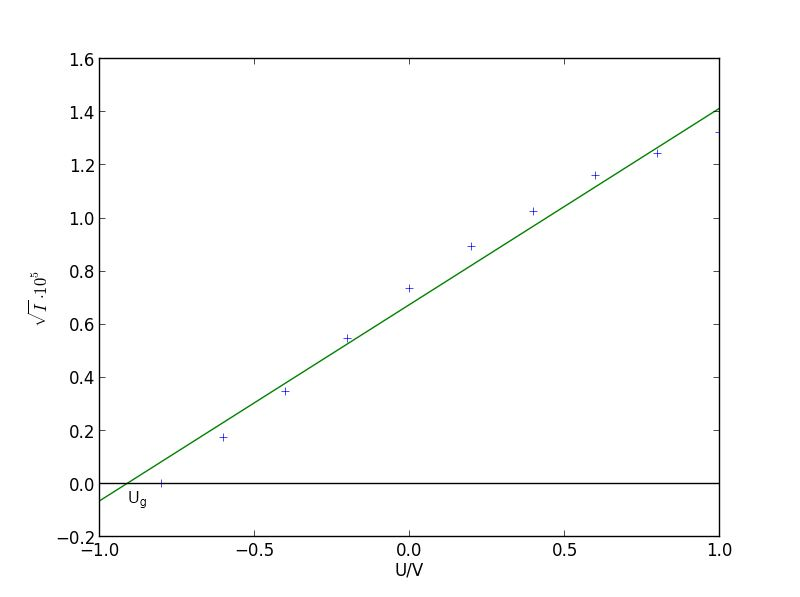
\includegraphics[scale=0.7]{picablaugrunlin.jpg}
		\caption{Lineare Regression des Photostroms ($\lambda=492$ nm)}
		\label{picablaugrunlin}
		\end{center}	
	\end{figure} 	\begin{figure}[h]
		\begin{center}
		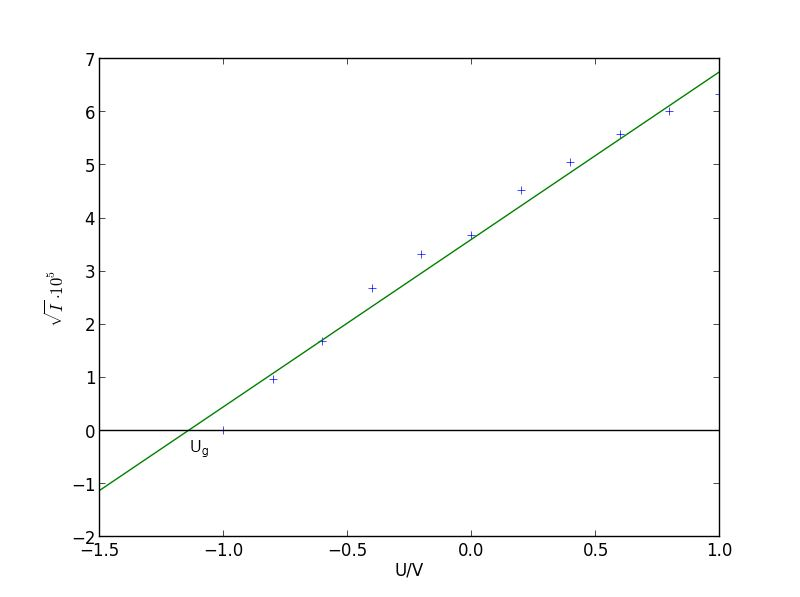
\includegraphics[scale=0.7]{picavio1lin.jpg}
		\caption{Lineare Regression des Photostroms ($\lambda=435$ nm)}
		\label{picavio1lin}
		\end{center}	
	\end{figure} 	\begin{figure}[h]
		\begin{center}
		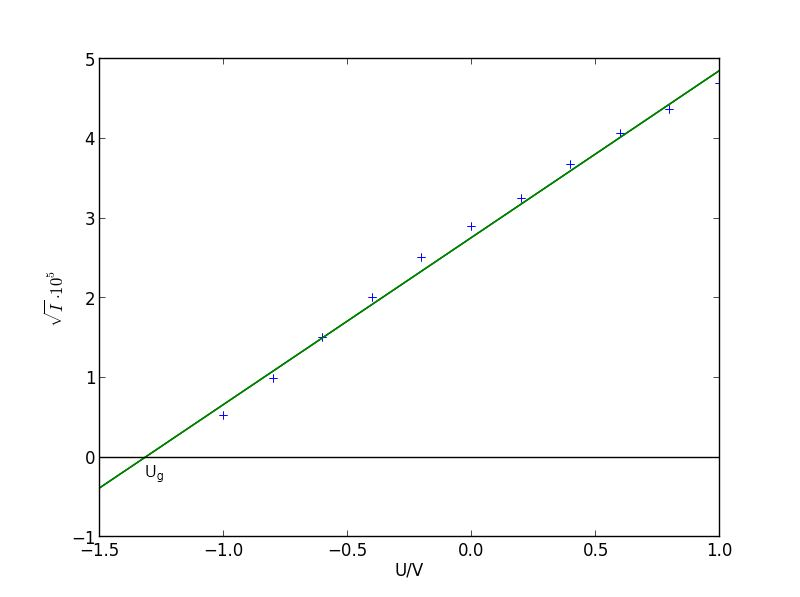
\includegraphics[scale=0.7]{picavio2lin.jpg}
		\caption{Lineare Regression des Photostroms ($\lambda=405$ nm)}
		\label{picavio2lin}
		\end{center}	
	\end{figure}
\begin{table}[h]
	\begin{center}
		\begin{tabular}{c|cc}
			$\lambda$/nm&a$\cdot 10^{-5}$&b$\cdot 10^{-5}$ \\ \hline
			405&2,10$\pm$0,06&2,77$\pm$0,04\\
			435&3,15$\pm$0,14&3,62$\pm$0,09\\
			492&0,74$\pm$0,03&0,68$\pm$0,02\\
			546&3,00$\pm$0,25&1,93$\pm$0,14\\
			578&2,18$\pm$0,16&1,03$\pm$0,09
		\end{tabular}
		\caption{Ergebnisse der linearen Regression}
		\label{tabalinreg}
	\end{center}
\end{table} \begin{table}[h]
	\begin{center}
		\begin{tabular}{cc}
			$U_g$/V&$\lambda$/nm \\ \hline
			-1,3202&405\\
			-1,1471&435\\
			-0,9163&492\\
			-0,6430&546\\
			-0,4733&578
		\end{tabular}
		\caption{$U_g$ in Abhängigkeit der Wellenlänge}
		\label{tabug}
	\end{center}
\end{table}
%\FloatBarrier
Wird die Wurzel aus dem Photostrom gegen die Bremsspannung aufgetragen, so lässt sich
für die verschiedenen Wellenlängen (vgl. Tab. \ref{tabspektrum}) aus den Tabellen \ref{tabaall} und \ref{tabay} Abbildung \ref{picaALL}
erstellen. Wird nun für die linearen Abschnitte aus Abbildung \ref{picaALL} jeweils eine lineare 
Regression \cite{linreg} durchgeführt (siehe Tab. \ref{tabalinreg}), 
\begin{align}
\sqrt{I}&=a\cdot U+b,
\end{align}
so lassen
sich aus dem Schnittpunkt der Ausgleichsgeraden mit der Spannungs-Achse (Abb. \ref{picagelblin} - 
\ref{picavio2lin}) die Gegenspannungen $U_g$ bestimmen.
\begin{align}
U_g&=\frac{-b}{a}
\end{align}

\subsection{Bestimmung der Austrittsarbeit und des Verhältnisses $\frac{h}{e_0}$}
	\begin{figure}[h]
		\begin{center}
		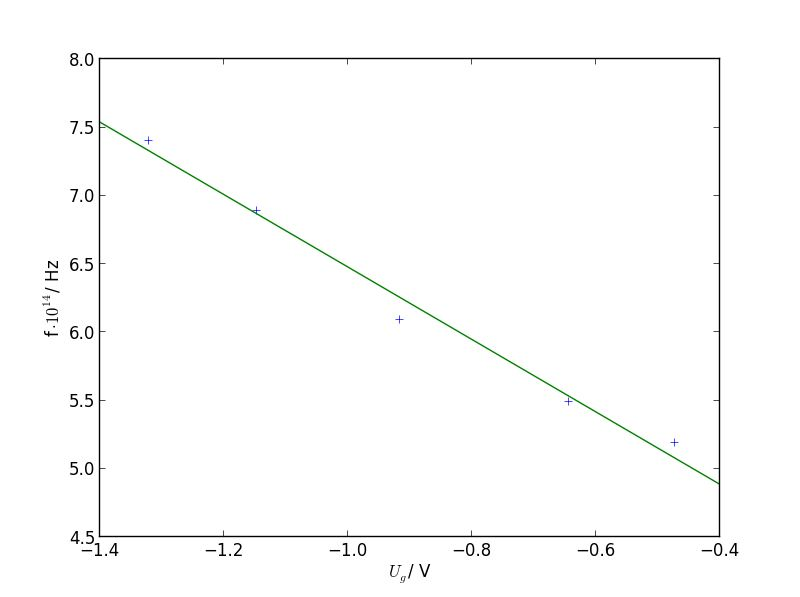
\includegraphics[scale=0.7]{picblinreg1.jpg}
		\caption{Lineare Regression von $U_g$ bezogen auf die Lichtfrequenz}
		\label{picblinreg1}
		\end{center}	
	\end{figure}
Wird $U_g$ (Tab. \ref{tabug}) gegen die Lichtfrequenz (Tab. \ref{tabspektrum}) aufgetragen 
(Abb. \ref{picblinreg1}) und dann ein lineare Regression \cite{linreg} durchgeführt, so 
lassen sich Austrittsarbeit $A_k$ und das Verhältnis $\frac{h}{e_0}$ mit Gleichung (\ref{equg}) 
bestimmen.
\begin{align}
\nu &= \frac{e_0}{h} |U_g| + \frac{A_k}{h}\\
\frac{A_k}{h}&=(3,8\pm0,2)\cdot10^{14}\text{ }\frac{1}{s}\\
\Rightarrow A_k&=(1,58\pm0,07)\text{ eV}\\
\frac{h}{e_0}&=((2,6 \pm 0,2)\cdot 10^{14} \text{ } \frac{\text{C}}{\text{J}\cdot \text{s}})^{-1}=(3,8\pm0,3)\cdot10^{-15}\text{ }\frac{\text{J$\cdot$s}}{\text{C}}
\end{align}


% \subsection{Deutung eines Kurvenverlaufs}
% 	\begin{figure}[h]
		\begin{center}
		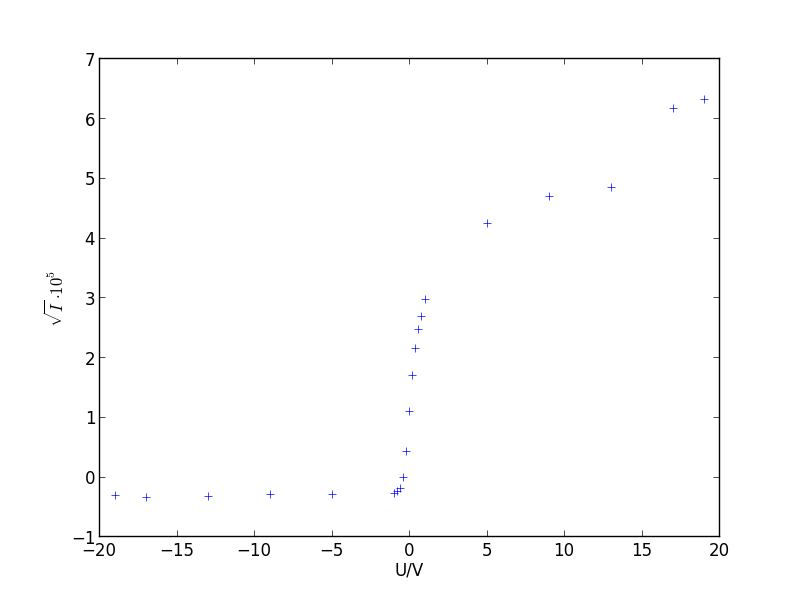
\includegraphics[scale=0.7]{picagelb.jpg}
		\caption{Photostrom in Abhängigkeit der angelegten Spannung ($\lambda=492$ nm)}
		\label{picagelb}
		\end{center}	
	\end{figure}
% In Abbildung \ref{picagelb} ist für $\lambda=578\text{ nm}$ der Photostrom abhängig der
% angelegten Spannung aufgetragen. Es ist bei hohen beschleunigenden Spannungen ein
% Sättigungsverhalten zu erkennen, dem zu Grunde liegt die Eigenschaft, dass die Anzahl der
% ausgelösten Elektronen von der Intesität des Lichtes abhängt. Das Ohmschen Gesetz lässt sich in diesem Fall 
% nicht anwenden, da die Elektronen zur Anode hin beschleunigt werden. Dieser Sättigungswert hängt neben
% der Intensität des Lichtes auch von der bestrahlten Fläche und den Materialeigenschaften ab. Dabei liegt 
% die Asymptotik an dem Unvermögen der Versuchsanordnung alle Elektronen zu registrieren, damit wirklich 
% alle Elektronen die Anode erreichen, müsste der Abstand zwischen Anode und Kathode gegen Null
% streben, was natürlich ein solches Experiment unmöglich machen würde.\\ 
% Der Photostrom nähert sich bereits bei $U>U_g$ an 0 V an, da die Elektronen nach der Fermi-Dirac 
% Statistik verteilt sind und es so auch Elektronen gibt, die bei $U>U_g$ gar nicht erst genug
% Energie besitzen die Anode zu erreichen. Der entgegengerichtete Photostrom von ungefähr -0,01 nA 
% kommt durch den an der Anode stattfindenden Photoeffekt zustande. Da die bestrahlte Oberfläche der 
% Anode wesentlich kleiner ist, wird schon bei relativ kleinen Spannungsbeträgen eine Sättigung erreicht.
% Die Austrittsarbeit der Anode ist gering, denn schon bei Einstrahlung energiearmen Lichtes 
% ($\lambda \approx 650$ nm)\cite{anleitung} tritt bereits ein negativer Photostrom auf.